\documentclass{report}
\usepackage[utf8]{inputenc}

\usepackage{cite}
\usepackage{amsmath}
\usepackage{amssymb}
\usepackage[dvipsnames]{xcolor}
\usepackage[pdftex]{graphicx}
\usepackage{subcaption}
\usepackage{hyperref}
\hypersetup{
  colorlinks,
  linktoc=all
  citecolor=black,
  filecolor=black,
  linkcolor=black,
  urlcolor=black
}

% Linear algebra
\renewcommand{\Vec}[1]{{\mathbf{#1}}}
\newcommand{\Mat}[1]{{\mathbf{#1}}}
\newcommand{\real}{{\rm I\!R}}
\newcommand{\Zeros}[2]{{\Vec{0}_{#1\times#2}}}
\newcommand{\Norm}[1]{{\|#1\|}}
\newcommand{\I}{{\Mat{I}}}
\newcommand{\quat}{{\Vec{q}}}
\newcommand{\jac}{{\Mat{J}}}
\newcommand{\Skew}[1]{{\lfloor #1 \enspace \times \rfloor}}
\newcommand{\Argmin}[1]{\underset{#1}{{\text{argmin }}}}
\newcommand{\Transpose}[1]{{{#1^{\top}}}}
\newcommand{\Inv}[1]{{{#1^{-1}}}}

% Frames
\newcommand{\tf}{\mathbf{T}}
\renewcommand{\frame}{\mathcal{F}}
\newcommand{\body}{{\text{B}}}
\newcommand{\cam}{{\text{C}}}
\newcommand{\robot}{{\text{R}}}
\newcommand{\sensor}{{\text{S}}}
\newcommand{\world}{{\text{W}}}
\newcommand{\worldb}{{\text{G}}}
\newcommand{\fiducial}{{\text{F}}}
% -- Kinematic Notation --
% ---- Paul Furgale Kinematic Notation ----
\newcommand{\KineNotationTransform}[3]{{{#1}_{#2#3}}}
\newcommand{\KineNotation}[3]{{{{}_{#2}} {#1}_{#2#3}}}
\newcommand{\KineNotationPart}[3]{{{{}_{#2}} {#1}_{#3}}}
\newcommand{\KineNotationBare}[2]{{{{}_{#2}} {#1}}}
% -- Translation --
\newcommand{\trans}{{\Vec{r}}}
\newcommand{\Trans}[2]{{\KineNotation{\trans}{#1}{#2}}}
% -- Position --
\newcommand{\pos}{{\Vec{r}}}
\newcommand{\Pos}[2]{{\KineNotation{\pos}{#1}{#2}}}
% -- Velocity --
\newcommand{\vel}{{\Vec{v}}}
\newcommand{\Vel}[2]{{\KineNotation{\vel}{#1}{#2}}}
% -- Angular Velocity --
\newcommand{\angvel}{{\boldsymbol{\omega}}}
\newcommand{\AngVel}[2]{{\KineNotation{\angvel}{#1}{#2}}}
% -- Acceleration --
\newcommand{\acc}{{\Vec{a}}}
\newcommand{\Acc}[2]{{\KineNotation{\acc}{#1}{#2}}}
% -- Rotation --
\newcommand{\dtheta}{{\delta{\boldsymbol{\theta}}}}
\newcommand{\rot}{{\Mat{C}}}
\newcommand{\Rot}[2]{{\KineNotationTransform{\rot}{#1}{#2}}}
% -- Transforms --
\newcommand{\tf}{{\Mat{T}}}
\newcommand{\Tf}[2]{{\KineNotationTransform{\tf}{#1}{#2}}}
% -- Point --
\newcommand{\point}{\Vec{p}}
\newcommand{\Pt}[1]{{\KineNotationPart{\point}{#1}{}}}
\newcommand{\Point}[2]{{\KineNotationBare{\point}{#1}}}

% Variables
\newcommand{\error}{{\Vec{e}}}
\newcommand{\camRot}{{\Rot{\world}{\cam}}}
\newcommand{\camPos}{{\Pos{\world}{\cam}}}
\newcommand{\projFunc}{{\Vec{h}}}
\newcommand{\measurement}{{\Vec{z}}}
\newcommand{\estimate}{{\tilde{\Vec{z}}}}


\begin{document}

% TABLE OF CONTENTS
\tableofcontents

% CHAPTERS
\chapter{Notations}

A large part of robotics is about developing machines that perceives and
interact with the environment. For that robots use sensors to collect and
process data, and knowing what the data describes is of utmost importance.
Imagine obtaining the position of the robot but not knowing what that position
is with respect to. Missing data descriptions such as what a position vector is
expressing, what is it with respect to and more causes many hours of painful
trail and error to extract that information.

In the following section the notation used throughout this document will be
described, and it follows closely of that of Paul Furgale's~\cite{Furgale2014}.
The aim is to mitigate the ambiguity that arises when describing robot poses,
sensor data and more.

A vector expressed in the world frame, $\frame_{\world}$, is written as
$\KineNotationBare{\pos}{\world}$. Or more precisely if the vector describes
the position of the camera frame, $\frame_{\cam}$, expressed in
$\frame_{\world}$, the vector can be written as $\Pos{\world}{\cam}}$ with
$\world$ and $\cam$ as start and end points. The left hand subscripts indicates
the coordinate system the vector is expressed in, while the right-hand
subscripts indicate the start and end points. For brevity if the vector has
the same start point as the frame to which it is expressed in, the same vector
can be written as $\KineNotationPart{\pos}{\world}{\cam}$. Similarly a
transformation of a point from $\frame_{\cam}$ to $\frame_{\world}$ can be
represented by a homogeneous transform matrix, $\Tf{\world}{\cam}$, where its
rotation matrix component is written as $\Rot{\world}{\cam}$ and the
translation component written as $\Trans{\world}{\cam}$. A rotation matrix that
is parametrized by quaternion $\quat_{\world\cam}$ is written as
$\rot\{\quat_{\world\cam}\}$.



\begin{align*}
  &\text{Position:} \enspace & \Pos{\world}{\body} \\
  &\text{Velocity:} \enspace & \Vel{\world}{\body} \\
  &\text{Acceleration:} \enspace & \Acc{\world}{\body} \\
  &\text{Angular velocity:} \enspace & \AngVel{\world}{\body} \\
  &\text{Rotation:} \enspace & \Rot{\world}{\body} \\
  &\text{Transform:} \enspace & \Tf{\world}{\body} \\
  &\text{Point:} \enspace & \Pt{\world}
\end{align*}

\chapter{Rotations}

\section{Euler Angles}
Z-Y-X rotation sequence:

\begin{equation}
  \rot_{zyx} =
  \begin{bmatrix}
    c(\psi) c(\theta)
    & c(\psi) s(\theta) s(\phi) - s(\psi) c(\phi)
    & c(\psi) s(\theta) c(\phi) + s(\psi) s(\phi) \\
    s(\psi) c(\theta)
    & s(\psi) s(\theta) s(\phi) + c(\psi) c(\phi)
    & s(\psi) s(\theta) c(\phi) - c(\psi) s(\phi) \\
    -s(\theta) & c(\theta) s(\phi) & c(\theta) c(\phi)
  \end{bmatrix}
\end{equation}



% QUATERNIONS
\section{Quaternions}

A quaternion, $\Vec{q} \in \real^{4}$, generally has the following form
%
\begin{equation}
  \quat = q_{w} + q_{x} \mathbf{i} + q_{y} \mathbf{j} + q_{z} \mathbf{k},
\end{equation}
%
where $\{ q_{w}, q_{x}, q_{y}, q_{z} \} \in \real$ and $\{ \mathbf{i}, \mathbf{j},
\mathbf{k} \}$ are the imaginary numbers satisfying
%
\begin{equation}
\begin{split}
  &\mathbf{i}^{2}
  = \mathbf{j}^{2}
  = \mathbf{k}^{2}
  = \mathbf{ijk}
  = -1 \\
  \mathbf{ij} = -\mathbf{ji} &= \mathbf{k}, \enspace
  \mathbf{jk} = -\mathbf{kj} = \mathbf{i}, \enspace
  \mathbf{ki} = -\mathbf{ik} = \mathbf{j}
\end{split}
\end{equation}
%
corresponding to the Hamiltonian convention. The quaternion can be written as a
4 element vector consisting of a \textit{real} (\textit{scalar}) part, $q_{w}$,
and \textit{imaginary} (\textit{vector}) part $\quat_{v}$ as,
%
\begin{equation}
  \quat =
  \begin{bmatrix} q_{w} \\ \quat_{v} \end{bmatrix} =
  \begin{bmatrix} q_{w} \\ q_{x} \\ q_{y} \\ q_{z} \end{bmatrix}
\end{equation}
%
There are other quaternion conventions, for example, the JPL convention. A more
detailed discussion between Hamiltonian and JPL quaternion convention is
discussed in \cite{Sola2017}.


\subsection{Main Quaternion Properties}
\subsubsection{Sum}

Let $\Vec{p}$ and $\Vec{q}$ be two quaternions, the sum of both quaternions is,
%
\begin{equation}
  \Vec{p} \pm \Vec{q} =
  \begin{bmatrix} p_w \\ \Vec{p}_{v} \end{bmatrix}
  \pm
  \begin{bmatrix} q_w \\ \Vec{q}_{v} \end{bmatrix} =
  \begin{bmatrix} p_w \pm q_w \\ \Vec{p}_{v} \pm \Vec{q}_{v} \end{bmatrix}.
\end{equation}
%
The sum between two quaternions $\Vec{p}$ and $\Vec{q}$ is \textbf{commutative}
and \textbf{associative}.
%
\begin{equation}
  \Vec{p} + \Vec{q} = \Vec{q} + \Vec{p}
\end{equation}
%
\begin{equation}
  \Vec{p} + (\Vec{q} + \Vec{r}) = (\Vec{p} + \Vec{q}) + \Vec{r}
\end{equation}


\subsubsection{Product}

The quaternion multiplication (or product) of two quaternions $\Vec{p}$ and
$\Vec{q}$, denoted by $\otimes$ is defined as
%
\begin{align}
  \Vec{p} \otimes \Vec{q}
    &=
    (p_w + p_x \mathbf{i} + p_y \mathbf{j} + p_z \mathbf{k})
    (q_w + q_x \mathbf{i} + q_y \mathbf{j} + q_z \mathbf{k}) \\
    &=
    \begin{matrix}
      &(p_w q_w - p_x q_x - p_y q_y - p_z q_z)& \\
      &(p_w q_x + p_x q_w + p_y q_z - p_z q_y)& \mathbf{i}\\
      &(p_w q_y - p_y q_w + p_z q_x + p_x q_z)& \mathbf{j}\\
      &(p_w q_z + p_z q_w - p_x q_y + p_y q_x)& \mathbf{k}\\
    \end{matrix} \\
    &=
    \begin{bmatrix}
      \label{eq:quaternion_product}
      p_w q_w - p_x q_x - p_y q_y - p_z q_z \\
      p_w q_x + q_x p_w + p_y q_z - p_z q_y \\
      p_w q_y - p_y q_w + p_z q_x + p_x q_z \\
      p_w q_z + p_z q_w - p_x q_y + p_y q_x \\
    \end{bmatrix} \\
    &=
    \begin{bmatrix}
      \label{eq:quaternion_product_2}
      p_w q_w - \Transpose{\Vec{p}_{v}} \Vec{q}_{v} \\
      p_w \Vec{q}_{v} + q_w \Vec{p}_{v} + \Vec{p}_{v} \times \Vec{q}_{v}
    \end{bmatrix}.
\end{align}
%
The quaternion product is \textbf{not commutative} in the general
case\footnote{There are exceptions to the general non-commutative rule, where
either $\Vec{p}$ or $\Vec{q}$ is real such that $\Vec{p}_{v} \times \Vec{q}_{v}
= 0$, or when both $\Vec{p}_v$ and $\Vec{q}_v$ are parallel, $\Vec{p}_v ||
\Vec{q}_v$. Only in these cirmcumstances is the quaternion product
commutative.},
%
\begin{equation}
  {\Vec{p} \otimes \Vec{q} \neq \Vec{q} \otimes \Vec{p}} \enspace .
\end{equation}
%
The quaternion product is however \textbf{associative},
%
\begin{equation}
  \Vec{p} \otimes (\Vec{q} \otimes \Vec{r})
  = (\Vec{p} \otimes \Vec{q}) \otimes \Vec{r}
\end{equation}
%
and \textbf{distributive over the sum}
%
\begin{equation}
  \Vec{p} \otimes (\Vec{q} + \Vec{r}) =
  \Vec{p} \otimes \Vec{q} + \Vec{p} \otimes \Vec{r}
  \quad \text{and} \quad
  (\Vec{p} \otimes \Vec{q}) + \Vec{r} =
  \Vec{p} \otimes \Vec{r} + \Vec{q} \otimes \Vec{r}
\end{equation}

The quaternion product can alternatively be expressed in matrix form as
%
\begin{equation}
  \Vec{p} \otimes \Vec{q} = [\Vec{p}]_{L} \Vec{q}
  \quad \text{and} \quad
  \Vec{p} \otimes \Vec{q} = [\Vec{q}]_{R} \Vec{p} \enspace ,
\end{equation}
%
where $[\Vec{p}]_{L}$ and $[\Vec{q}]_{R}$ are the left and right
quaternion-product matrices which are derived from
\eqref{eq:quaternion_product},
%
\begin{equation}
  [\Vec{p}]_{L} =
  \begin{bmatrix}
    p_w & -p_x & -p_y & -p_z \\
    p_x & p_w & -p_z & p_y \\
    p_y & p_z & p_w & -p_x \\
    p_z & -p_y & p_x & p_w
  \end{bmatrix},
  \quad \text{and} \quad
  [\Vec{q}]_{R} =
  \begin{bmatrix}
    q_w & -q_x & -q_y & -q_z \\
    q_x & q_w & q_z & -q_y \\
    q_y & -q_z & q_w & q_x \\
    q_z & q_y & -q_x & q_w
  \end{bmatrix},
\end{equation}
%
or inspecting \eqref{eq:quaternion_product_2} a compact form can be derived as,
%
\begin{equation}
  [\Vec{p}]_{L} =
  \begin{bmatrix}
    0 & -\Transpose{\Vec{p}_{v}} \\
    \Vec{p}_w \I_{3 \times 3} + \Vec{p}_{v} &
    \Vec{p}_w \I_{3 \times 3} -\Skew{\Vec{p}_{v}}
  \end{bmatrix}
\end{equation}
%
and
%
\begin{equation}
  [\Vec{q}]_{R} =
  \begin{bmatrix}
    0 & -\Transpose{\Vec{q}_{v}} \\
    \Vec{q}_w \I_{3 \times 3} + \Vec{q}_{v} &
    \Vec{q}_w \I_{3 \times 3} -\Skew{\Vec{q}_{v}}
  \end{bmatrix},
\end{equation}
%
where $\Skew{\bullet}$ is the skew operator that produces a matrix cross
product matrix, and is defined as
%
\begin{equation}
  \Skew{\Vec{v}} =
  \begin{bmatrix}
    0 & -v_{3} & v_{2} \\
    v_{3} & 0 & -v_{1} \\
    -v_{2} & v_{1} & 0
  \end{bmatrix},
  \quad
  \Vec{v} \in \real^{3}
\end{equation}
%

\subsubsection{Conjugate}

The conjugate operator for quaternion, ${(\bullet)}^{\ast}$, is
defined as
%
\begin{equation}
  \quat^{\ast}
  =
  \begin{bmatrix}
    q_w \\
    - \Vec{q}_v
  \end{bmatrix}
  =
  \begin{bmatrix}
    q_w \\
    - q_x \\
    - q_y \\
    - q_z
  \end{bmatrix}.
\end{equation}
%
This has the properties
%
\begin{equation}
  \quat \otimes \quat^{-1}
  = \quat^{-1} \otimes \quat
  = q_{w}^{2} + q_{x}^{2} + q_{y}^{2} + q_{z}^{2}
  =
  \begin{bmatrix}
    q_{w}^{2} + q_{x}^{2} + q_{y}^{2} + q_{z}^{2} \\
    \Vec{0}
  \end{bmatrix},
\end{equation}
%
and
%
\begin{equation}
  (\Vec{p} \otimes \Vec{q})^{\ast}
  = \Vec{q}^{\ast} \otimes \Vec{p}^{\ast}.
\end{equation}


\subsubsection{Norm}

The norm of a quaternion is defined by
%
\begin{align}
  \Norm{\quat} &= \sqrt{\quat \otimes \quat^{\ast}} \\
    &= \sqrt{\quat^{\ast} \otimes \quat} \\
    &= \sqrt{q_{w}^{2} + q_{x}^{2} + q_{y}^{2} + q_{z}^{2}}
    \enspace \in \real,
\end{align}
%
and has the property
%
\begin{align}
  \Norm{\Vec{p} \otimes \Vec{q}} =
  \Norm{\Vec{q} \otimes \Vec{p}} =
  \Norm{\Vec{p}} \Norm{\Vec{q}}
\end{align}



% -- QUATERNION FROM TWO VECTORS
\subsection{Quaternion from Two Vectors}

% TODO: Need to reword the beginning
Using the properties of the cross and dot product
%
\begin{align}
  \Vec{u} \cdot \Vec{v} &=
    \Norm{\Vec{u}} \Norm{\Vec{v}} \cos \theta \\
  \Norm{\Vec{u} \times \Vec{v}} &=
    \Norm{\Vec{u}} \Norm{\Vec{v}} \Norm{\sin \theta} ,
\end{align}
%
the axis angle, $\boldsymbol{\theta} \in \real^{3}$, can be obtained from
$\Vec{u}$ and $\Vec{v}$ with
%
\begin{align}
  % -- Axis-angle
  \boldsymbol{\theta} &= \theta \Vec{e} \\
  % -- Angle
  \label{eq:angle_axis_calc_angle}
  \theta &= \cos^{-1}(
    \dfrac{\Vec{u} \cdot \Vec{v}}
          {\Norm{\Vec{u}} \Norm{\Vec{v}}}
  ) \quad , \enspace \theta \in \real \\
  % -- Axis
  \label{eq:angle_axis_calc_axis}
  \Vec{e} &=
    \dfrac{\Vec{u} \times \Vec{v}}{\Norm{\Vec{u} \times \Vec{v}}}
    \quad , \enspace \Vec{e} \in \real^{3}
\end{align}
%
where $\Vec{e}$ is the unit vector that defines the rotation axis and $\theta$
is the rotation angle about $\Vec{e}$. Once the axis angle,
$\boldsymbol{\theta}$, is obtained a quaternion can be formed
%
\begin{equation}
  \label{eq:quaternion_from_axis_angles}
  \quat =
    \cos \dfrac{\theta}{2}
    + \Vec{i} \sin \dfrac{\theta}{2} e_{x}
    + \Vec{j} \sin \dfrac{\theta}{2} e_{y}
    + \Vec{k} \sin \dfrac{\theta}{2} e_{z} \enspace .
\end{equation}


\subsubsection{Example: Attitude from gravity and accelerometer vectors}

In robotics knowing the attitude of the system is often required. An Inertial
Measurement Unit (IMU) is commonly used to obtain this information. Using the
method described previously, a gravity vector along with an accelerometer
measurement vector can be used to obtain an attitude in form of a quaternion.

Let $\Vec{g} \in \real^{3}$ be the gravity vector, and $\Vec{a}_{m} \in
\real^{3}$ be the accelerometer measurement from an IMU. With the two vectors
$\Vec{g}$ and $\Vec{a}_{m}$ a quaternion $\quat_{\world\sensor}$ expressing the
rotation of the IMU sensor frame, $\frame_{\sensor}$, with respect to the world
frame, $\frame_{\world}$, can be calculated given that values for $\Vec{g}$ and
$\Vec{a}_{m}$ are known. For example let
%
\begin{align}
  % -- Gravity vector
  \Vec{g} &= \Transpose{\begin{bmatrix} 0 & 0 & -9.81 \end{bmatrix}} \\
  % -- Accelerometer measurement vector
  \Vec{a}_{m} &= \Transpose{
    \begin{bmatrix}
      9.2681 &
      -0.310816 &
      -3.14984
    \end{bmatrix}
  } ,
\end{align}
%
taken from the first measurement of the \texttt{imu\_april} calibration
sequence of the EuRoC MAV dataset.

\begin{figure}[htp]
  \centering
  \begin{subfigure}[b]{0.47\textwidth}
    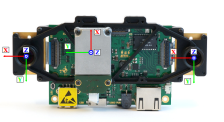
\includegraphics{images/quaternion/visensor_frames}
    \caption{VI-Sensor Coordinate Frames}
  \end{subfigure}
  ~ \quad
  \begin{subfigure}[b]{0.47\textwidth}
    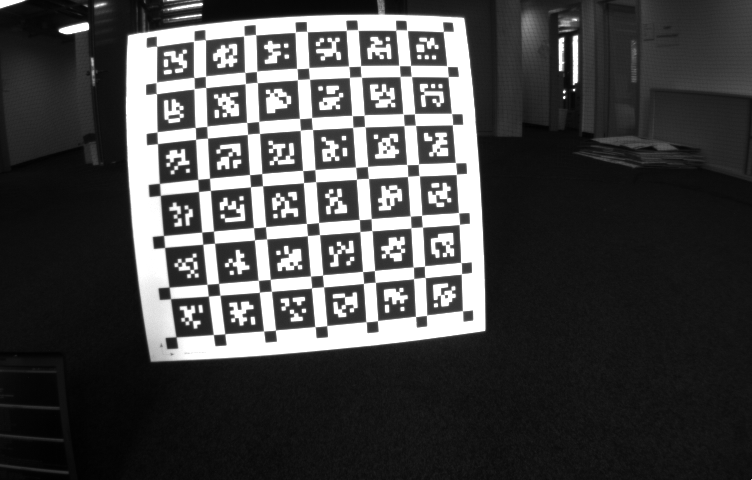
\includegraphics[width=\textwidth]{images/quaternion/1404733405732800000}
    \caption{Image frame}
  \end{subfigure}
  % \caption{EuRoC MAV Dataset - \begin{verbatim}imu_april\end{verbatim} sequence}
  \caption{EuRoC MAV Dataset - \texttt{imu\_april} Sequence}
\end{figure}

Before calculating the axis-angle, however, it should be noted that when an
accelerometer is at rest the measurement reading in the z-axis is positive
instead of negative. The reason is accelerometers measures acceleration by
measuring the displacement of a proof mass that is suspended with springs. For
example, if gravity is ignored and the accelerometer moves upwards, the proof mass
will be displaced towards the bottom of the accelerometer. This is interpreted
as an acceleration in the upwards direction, and so when the accelerometer is
at rest on a flat surface, gravity pulls on the proof mass yeilding a positive
measurement in the upwards direction. To resolve this issue the gravity vector
is negated, and so $\Vec{u} = -\Vec{g}$ and $\Vec{v} = \Vec{a}_{m}$. Using 
\eqref{eq:angle_axis_calc_angle} and \eqref{eq:angle_axis_calc_axis} the
axis-angle, $\boldsymbol{\theta}$, is thereby
%
\begin{align}
  % -- Axis-Angle
  \theta &= 1.8982 \\
  \Vec{e} &= \Transpose{
    \begin{bmatrix}
      0.03352 &
      0.99944 &
      0.00000
    \end{bmatrix}
  }
\end{align}
%
Finally the quaternion, $\quat_{\world\sensor}$, can be calculated using
\eqref{eq:quaternion_from_axis_angles} resulting in
%
\begin{equation}
  % -- Quaternion
  \quat_{\world\sensor} &= \Transpose{
    \begin{bmatrix}
      0.58240 &
      0.02725 &
      0.81245 &
      0.00000
    \end{bmatrix}
  } \enspace .
\end{equation}



% -- QUATERNION TO ROTATION MATRIX
\subsection{Quaternion to Rotation Matrix}

\begin{equation}
  \Mat{R}\{\quat \} = \begin{bmatrix}
    q_w^2 + q_x^2 - q_y^2 - q_z^2
    & 2(q_x q_y - q_w q_z)
    & 2(q_x q_z + q_w q_y) \\
    2(q_x q_y + q_w q_z)
    & q_w^2 - q_x^2 + q_y^2 - q_z^2
    & 2(q_y q_z - q_w q_x) \\
    2(q_x q_y - q_w q_y)
    & 2(q_y q_z + q_w q_x)
    & q_w^2 - q_x^2 - q_y^2 + q_z^2
  \end{bmatrix}
\end{equation}



% DIFFERENTIAL CALCULUS OF 3D CALCULUS
\section{Differential Calculus}

Lie Group $SO(3)$
\begin{itemize}
  \item{Not a vector space}
  \item{Has no addition operator
  \item{Has no subtraction operator
\end{itemize}

State estimation frameworks rely on small differences and gradients in order to
correct the state estimate. Orientations unlike translation and velocity do not
have an addition operator, as such it is more involving to update or
find the gradients of orientations. Forunately, since orientations are a
special orhogonal group $SO(3)$ as well as a Lie group, an exponential map
exists that relates to its Lie algebra allowing orientations to be perturbed
and its gradients calculated.

Elements in Lie algebra are abstract vectors and not suitable for actual
computations. A basis $\mathbf{B} = [\vec{\boldsymbol{\varphi}}_{1} \enspace
\vec{\boldsymbol{\varphi}}_{2} \enspace \vec{\boldsymbol{\varphi}}_{3}]$
can be used to extend the map to $\real^{3}$. 

The definition of an exponential map $\text{exp} : \real^{3} \mapsto SO(3)$ of a
coordinate tuple $\boldsymbol{\varphi} (\varphi_1, \varphi_2, \varphi_3) \in
\real^{3}$ is defined by

\begin{equation}
  \text{exp}(\boldsymbol{\varphi}) := Exp(
    \vec{\boldsymbol{\varphi}}_{1}\varphi_{1},
    \vec{\boldsymbol{\varphi}}_{2}\varphi_{2},
    \vec{\boldsymbol{\varphi}}_{3}\varphi_{3}
  )
\end{equation}


$\forall t, s \in \real$, $\forall \vec{\boldsymbol{\varphi}} \in $

\begin{align}
  Exp((t + s) \vec{\boldsymbol{\varphi}}) =
    Exp(t\vec{\boldsymbol{\varphi}}) \circ Exp(s\vec{\boldsymbol{\varphi}})
\end{align}


\begin{align}
  \boxplus :& SO(3) \times \real^{3} \rightarrow SO(3), \\
    &\Phi, \boldsymbol{\varphi}
      \mapsto \text{exp}(\boldsymbol{\varphi}) \circ \Phi, \nonumber \\
  \boxminus :& SO(3) \times SO(3) \rightarrow \real^{3}, \\
    &\Phi_1, \Phi_2 \mapsto \text{log}(\Phi_1 \circ \Phi_{2}^{-1}) \nonumber
\end{align}

Similar to regular addition and subtraction, both operators have the following
identities,
%
\begin{align}
  \Phi \boxplus \Vec{0} &= \Phi \\
  (\Phi \boxplus \boldsymbol{\varphi}) \boxminus \Phi &= \boldsymbol{\varphi} \\
  \Phi_1 \boxplus (\Phi_2 \boxminus \Phi_1) &= \Phi_2
\end{align}

\chapter{Computer Vision}

\subsection{Point on Line}

\begin{equation}
  \Transpose{\Vec{x}} \Vec{l} = 0
\end{equation}


\subsection{Intersection of Lines}

\begin{equation}
  \Vec{l} (\Vec{l} \times \Vec{l}')
  \Vec{l}' (\Vec{l} \times \Vec{l}')
  = 0 \\
  \Transpose{\Vec{l}} \Vec{x}
  = \Transpose{\Vec{l}}' \Vec{x}
  = 0
\end{equation}

\begin{equation}
  x = \Vec{l} \times \Vec{l}'
\end{equation}


\subsection{Plane}

\begin{itemize}
  \item{A plane can be defined by the join between three points, or the join
        between a line and a point in general}
  \item{Two planes intersecting a unique line}
  \item{Three planes intersecting a unique point}
\end{itemize}

\subsubsection{Three Points Define a Plane}

Suppose you have three points $\Vec{X}_{1}$, $\Vec{X}_{2}$, $\Vec{X}_{3}$, and
are incident with a plane, $\pi$ then each point satisfies
%
\begin{equation}
  \Transpose{\pi} \Vec{X}_{i} = 0.
\end{equation}
%
By stacking each point as a matrix
%
\begin{align}
  \begin{bmatrix}
    \Transpose{\Vec{X}_{1}} \\
    \Transpose{\Vec{X}_{2}} \\
    \Transpose{\Vec{X}_{3}}
  \end{bmatrix} \pi = 0
\end{align}
%
Since three points in general rare linearly independent, it follows that the
$3x4$ matrix compsed of the points $\Vec{X}_{i}$ as rows has rank 3.



% PINHOLE CAMERA MODEL
\section{Pinhole Camera Model}

\begin{equation}
  K =
  \begin{bmatrix}
    f_x & 0 & c_x \\
    0 & f_y & c_y \\
    0 & 0 & 1
  \end{bmatrix}
\end{equation}



% PINHOLE CAMERA MODEL
\section{Radial Tangential Distortion}

\begin{align}
\begin{split}
  k_{\text{radial}} &= 1 + (k_1 r^2) + (k_2 r^4) \\
  x' &= x \cdot k_{\text{radial}} \\
  y' &= y \cdot k_{\text{radial}} \\
  x'' &= x' + (2 p_1 x y + p_2 (r^2 + 2 x^2)) \\
  y'' &= y' + (p_1 (r^2 + 2 y^2) + 2 p_2 x y)
\end{split}
\end{align}



\section{Equi-distant Distortion}

\begin{align}
\begin{split}
  r &= \sqrt{x^{2} + y^{2}} \\
  \theta &= \arctan{(r)} \\
  \theta_d &= \theta (1 + k_1 \theta^2 + k_2 \theta^4 + k_3 \theta^6 + k_4 \theta^8) \\
  x' &= (\theta_d / r) \cdot x \\
  y' &= (\theta_d / r) \cdot y
\end{split}
\end{align}



% FEATURE ESTIMATION
\section{Feature Estimation}
\label{sec:feature_estimation}

In the previous section we have discussed methods to detect and match between
different camera frames. In this section we introduce a method to estimate
feature positions in 3D using 2D pixels measurements of the same feature in
different camera frames.

\subsection{Feature Initialization}
\label{subsec:linear_triangulation}

There are various methods for initializing the feature position. The linear
triangulation method~\cite{Hartley2003} is frequently used. This method assumes
a pair of homogeneous pixel measurements $\measurement$ and $\measurement' \in
\real^{3}$ that observes the same feature, $\mathbf{X}$, in homogeneous
coordinates from two different camera frames. The homogeneous projection from
3D to 2D with a known camera matrix $\Mat{P} \in \real^{3 \times 4}$
for each measurement is given as,
%
\begin{align}
\begin{split}
	\measurement &= \mathbf{P} \mathbf{X} \\
	\measurement' &= \mathbf{P}' \mathbf{X}.
\end{split}
\end{align}
%
These equations can be combined to form a system of equations of the form
$\Mat{A} \Vec{x} = 0$. To eliminate the homogeneous scale factor we apply a
cross product to give three equations for each image point, for example
$\measurement \times (\Mat{P} \Mat{X}) = \Vec{0}$ writing this out gives
%
\begin{align}
\label{eq:linear_triangulation_derivation}
\begin{split}
  x (\Vec{p}^{3T} \Vec{X}) - (\Vec{p}^{1T} \Vec{X}) = 0 \\
  y (\Vec{p}^{3T} \Vec{X}) - (\Vec{p}^{2T} \Vec{X}) = 0 \\
  x (\Vec{p}^{2T} \Vec{X}) - y (\Vec{p}^{1T} \Vec{X}) = 0
\end{split}
\end{align}
%
where $\Vec{p}^{iT}$ is the $i^{\mbox{th}}$ row of $\Vec{P}$.

From Eq.~\eqref{eq:linear_triangulation_derivation}, an equation of the form
$\Mat{A} \Vec{x} = \Vec{0}$ for each image point can be formed, where
$\Vec{x}$ represents the unknown homogeneous feature location to be
estimated, and $\Mat{A}$ is given as
%
\begin{align}
  \mathbf{A} =
  \begin{bmatrix}
    x (\Vec{p}^{3T}) - (\Vec{p}^{1T}) \\
    y (\Vec{p}^{3T}) - (\Vec{p}^{2T}) \\
    x' (\Vec{p'}^{3T}) - (\Vec{p'}^{1T}) \\
    y' (\Vec{p'}^{3T}) - (\Vec{p'}^{2T})
  \end{bmatrix}
  \label{eq:linear_triangulation_ derivation}
\end{align}
%
giving a total of four equations in four homogeneous unknowns. Solving for
$\Vec{A}$ using SVD allows us to estimate the initial feature location.


\subsection{Feature Refinement}
\label{subsec:bundle_adjustment}

The linear triangulation provides an initial feature position. In an ideal
world, feature positions can be solved as a system of equations. In reality,
however, errors are present in the camera poses and pixel measurements. The
pixel measurements observing the same 3D point are generally noisy. In
addition, the pinhole camera model and radial-tangential distortion model do
not perfectly model the camera projection or distortion observed. Therefore an
iterative method can be used to further refine the feature position. This
problem is generally formulated as a non-linear least square problem and can be
solved by numerical methods, such as the Gauss-Newton algorithm.

Let us consider the case where two different cameras at known locations observe
the same feature in the scene. Our goal is to optimize for the feature
position. With an $i^{\text{th}}$ feature measurement, and corresponding
$i^{\text{th}}$ camera orientation as a quaternion, $\quat_{\cam_{i}\world}$ and
$i^{\text{th}}$ camera position, $\pos_{\cam_{i}}^{\cam_{i}\world}$, we can
formulate the re-projection error as,
%
\begin{equation}
	\label{eq:bundle_adjustment_residual}
	\mathbf{e}_{i}(\boldsymbol{\theta},
								 \quat_{\cam_{i}\world},
								 \pos_{\cam_{i}}^{\cam_{i}\world})
	=
	\measurement_{i}
	- \mathbf{h}(\boldsymbol{\theta},
							 \quat_{\cam_{i}\world},
							 \pos_{\cam_{i}}^{\cam_{i}\world}).
\end{equation}
%
where the parameter, $\boldsymbol{\theta} \in \real^{3}$, represents the
feature location to be optimized, $\measurement_{i} \in \real^{2}$ is the
$i$-th pixel measurement, and $\mathbf{h} : \real^{10} \mapsto \real^{2}$ is
the projection function that projects $\boldsymbol{\theta}$ into the
measurement space using known camera extrinsics. The re-projection error is a
geometric error corresponding to the Euclidean distance between measured and
projected features onto the image plane, it is used for quantifying the error
of the estimated feature location. With the error function, $\Vec{e}_{i}$,
for one measurement, a cost function, $\Vec{f}$, for $m$ number of pixel
measurements in the form of sum of squares can be defined as,
%
\begin{equation}
  \label{eq:sfm}
  \mathbf{f}(\boldsymbol{\theta})
	= \sum^{m}_{i=1}
    \mathbf{e}_{i}(
	    \boldsymbol{\theta},
	    \quat_{\cam_{i}\world},
	    \pos_{\cam_{i}}^{\cam_{i}\world}
	)^{T}
	\mathbf{e}_{i}(
		\boldsymbol{\theta},
		\quat_{\cam_{i}\world},
		\pos_{\cam_{i}}^{\cam_{i}\world}
	).
\end{equation}
%
Now that the cost function, $\mathbf{f}(\boldsymbol{\theta})$, is defined an
unconstrained optimization can be performed using the cost function
Eq.~\ref{eq:sfm} to estimate the optimal feature position,
$\boldsymbol{\theta}^{*}$, which minimizes the re-projection error over the set
of collected measurements.
%
\begin{equation}
	\boldsymbol{\theta}^{*} = \argmin{\theta} \mathbf{f}(\boldsymbol{\theta}).
\end{equation}
%
%Note, to be clear, $\theta$ is usually the vector of all estimated parameters.
%This includes the camera pose, feature locations, and can also include
%calibration parameters.



\section{Bundle Adjustment}

Let $\measurement \in \re^{2}$ be the image measurement and $\projFunc(\cdot)
\in \re^{2}$ be the projection function that produces an image projection
$\estimate$. The reprojection error $e$ is defined as the euclidean distance
between $\measurement$ and $\estimate$.

\begin{equation}
  \error = \measurement - \estimate
\end{equation}

Our aim given image measurement $\measurement$ is to find the image projection
$\estimate$ that minimizes the reprojection $e$. The image projection
$\estimate$ in pixels can be represented in homogeneous coordinates with
$u, v, w$ as
%
\begin{equation}
  \estimate
  = \begin{bmatrix} x \\ y \end{bmatrix}
  = \begin{bmatrix} u / w \\ v / w \end{bmatrix}
\end{equation}
%
% Projection function
\begin{align}
  \label{eq:projection_function}
  \begin{bmatrix} u \\ v \\ w \end{bmatrix}
    = \Mat{P} \begin{bmatrix} \Pt{\world} \\ 1 \end{bmatrix}
      = \Mat{K} \camRot [\Pt{\world} - \camPos]
\end{align}
%
where $u, v, w$ is computed by projecting a landmark position $\Pt{\world}$ in
the world frame to the camera's image plane with projection matrix $\Mat{P}$.
The projection matrix, $\Mat{P}$, can be decomposed into the camera intrinsics
matrix, $\Mat{K}$, the camera rotation, $\camRot$, and camera position,
$\camPos$, expressed in the world frame.
%
The orientation of the camera in \eqref{eq:projection_function} is
represented using a rotation matrix. To reduce the optimization parameters
the rotation matrix can be parameterized by a quaternion by using the following
formula,
%
\begin{equation}
  \camRot = \begin{bmatrix}
    % Line 1
    q_{w}^{2} + q_{x}^{2} - q_{y}^{2} - q_{z}^{2}
    & 2 (q_{x} q_{y} - q_{w} q_{z})
    & 2 (q_{x} q_{z} + q_{w} q_{y}) \\
    % Line 2
    2 (q_{x} q_{y} + q_{w} q_{z})
    & q_{w}^{2} - q_{x}^{2} + q_{y}^{2} - q_{z}^{2}
    & 2 (q_{y} q_{z} - q_{w} q_{x}) \\
    % Line 3
    2 (q_{x} q_{z} - q_{w} q_{y})
    & 2 (q_{y} q_{z} + q_{w} q_{x})
    & q_{w}^{2} - q_{x}^{2} - q_{y}^{2} + q_{z}^{2}
  \end{bmatrix}.
\end{equation}
%
By parameterzing the rotation matrix with a quaternion, the optimization
parameters for the camera's orientation is reduced from 9 to 4.

Our objective is to optimize for the camera rotation $\camRot$, camera
position $\camPos$ and 3D landmark position $\Pt{\world}$ in order to
minimize the cost function,
%
\begin{align}
  &\Argmin{\camRot, \camPos, \Pt{\world}} \Norm{
    \measurement - \projFunc(\camRot, \camPos, \Pt{\world})
  }^{2} \\
  &\Argmin{\camRot, \camPos, \Pt{\world}} \Norm{
    \begin{bmatrix} x \\ y \end{bmatrix} -
    \begin{bmatrix} u / w \\ v / w \end{bmatrix}
    }^{2}.
\end{align}
%
The cost function above assumes only a single measurement, if there are $N$
measurements corresponding to $N$ unique landmarks the cost function can be
rewritten as a maximum likelihood estimation problem as,
%
\begin{equation}
  \Argmin{\camRot, \camPos, \Pt{\world}}
  \sum_{j = 1}^{N}
  \Norm{
    \measurement_{j} - \projFunc(\camRot^{j}, \camPos^{j}, \Point{\world}{j})
  }^{2}
\end{equation}
%
under the assumption that the observed landmark, $\Pt{\world}$, measured in
the image plane, $z$, are corrupted by a \textbf{zero-mean Gaussian noise}.

For the general case of $M$ images taken at different camera poses the cost
function can be further extended to,
%
\begin{equation}
  \min_{\camRot, \camPos, \Pt{\world}} 
  \sum_{i = 1}^{M} \sum_{j = 1}^{N}
  \Norm{
    \measurement_{i, j}
    - \projFunc(\camRot^{i}, \camPos^{i}, \Point{\world}{j})
  }^{2}
\end{equation}
%
The optimization process begins by setting the first image camera pose as world
origin, and subsequent $\camRot_{i}$ and $\camPos_{i}$ will be relative to the
first camera pose.


\subsection*{Jacobians}

The Jacobian for the optimization problem for a \textbf{single measurement} has
the form:
%
\begin{equation}
  \jac = \begin{bmatrix}
    \color{red}
    \dfrac{\partial{\projFunc}}{\partial \camRot}
    \color{cyan}
    \dfrac{\partial{\camRot}}{\partial{\quat}} \quad
    \color{Mulberry}
    \dfrac{\partial{\projFunc}}{\partial \camPos} \quad
    \color{blue}
    \dfrac{\partial{\projFunc}}{\partial \Pt{\world}}
  \end{bmatrix} \\
\end{equation}
%
If there are two measurements the Jacobian is stacked with the following
pattern:
%
\begin{equation}
  \jac = \begin{bmatrix}
    \text{Image 1}_{2 \times 7}
      & \Zeros{2}{7}
      & \text{3D Point}_{2 \times 3} \\
    \Zeros{2}{7}
      & \text{Image 2}_{2 \times 7}
      & \text{3D Point}_{2 \times 3}
  \end{bmatrix}
\end{equation}


% DERIVATION FOR dh / dR
\subsubsection*{Derivation for
$\color{red}
\dfrac{\partial{\projFunc}}{\partial{\camRot}}$}

\begin{align}
  \color{red}
  \dfrac{\partial{\projFunc}}{\partial{\camRot}} =
  \begin{bmatrix}
    \dfrac{
      w \dfrac{\partial{u}}{\partial{\camRot}} -
      u \dfrac{\partial{w}}{\partial{\camRot}}
    }{w^{2}} \vspace{1.0em} \\
    \dfrac{
      w \dfrac{\partial{v}}{\partial{\camRot}} -
      v \dfrac{\partial{w}}{\partial{\camRot}}
    }{w^{2}} \vspace{0.5em}
  \end{bmatrix}_{2 \times 9}
\end{align}

\begin{align}
  % Line 1
  \begin{bmatrix} u \\ v \\ w \end{bmatrix}
    &= \Mat{K} \camRot [\Pt{\world} - \camPos]
    \nonumber \\
  % Line 2
  \begin{bmatrix} u \\ v \\ w \end{bmatrix}
  &= \begin{bmatrix}
      f_x & 0 & p_x \\
      0 & f_y & p_y \\
      0 & 0 & 1
  \end{bmatrix}
  \begin{bmatrix}
      R_{11} & R_{12} & R_{13} \\
      R_{21} & R_{22} & R_{23} \\
      R_{31} & R_{32} & R_{33}
  \end{bmatrix}
  [\Pt{\world} - \camPos]
  \nonumber
\end{align}

\begin{align}
  \dfrac{\partial{u}}{\partial{\camRot}} &=
      \begin{bmatrix}
        f_{x} (\Pt{\world} - \camPos) &
        \Zeros{1}{3} &
        p_{x} (\Pt{\world} - \camPos)
      \end{bmatrix}_{1 \times 9} \\
  \dfrac{\partial{v}}{\partial{\camRot}} &=
    \begin{bmatrix}
      \Zeros{1}{3} &
      f_{y} (\Pt{\world} - \camPos) &
      p_{y} (\Pt{\world} - \camPos)
  \end{bmatrix}_{1 \times 9} \\
  \dfrac{\partial{w}}{\partial{\camRot}} &=
    \begin{bmatrix}
      \Zeros{1}{3} &
      \Zeros{1}{3} &
      (\Pt{\world} - \camPos)
    \end{bmatrix}_{1 \times 9}
\end{align}


% DERIVATION FOR dR / dq
\subsubsection*{Derivation for \color{cyan}
$\dfrac{\partial{\camRot}}{\partial{\quat}}$}

\begin{align}
  \color{cyan}
  \dfrac{\partial{\camRot}}{\partial{\quat}} =
  \begin{bmatrix}
    \dfrac{\partial{\camRot_{11}}}{\partial{\quat}} \\
    \dfrac{\partial{\camRot_{12}}}{\partial{\quat}} \\
    \vdots \\
    \dfrac{\partial{\camRot_{33}}}{\partial{\quat}}
  \end{bmatrix}_{9 \times 4}
\end{align}

\begin{equation}
  \camRot = \begin{bmatrix}
    % Line 1
    q_{w}^{2} + q_{x}^{2} - q_{y}^{2} - q_{z}^{2}
    & 2 (q_{x} q_{y} - q_{w} q_{z})
    & 2 (q_{x} q_{z} + q_{w} q_{y}) \\
    % Line 2
    2 (q_{x} q_{y} + q_{w} q_{z})
    & q_{w}^{2} - q_{x}^{2} + q_{y}^{2} - q_{z}^{2}
    & 2 (q_{y} q_{z} - q_{w} q_{x}) \\
    % Line 3
    2 (q_{x} q_{z} - q_{w} q_{y})
    & 2 (q_{y} q_{z} + q_{w} q_{x})
    & q_{w}^{2} - q_{x}^{2} - q_{y}^{2} + q_{z}^{2}
  \end{bmatrix}
  \nonumber
\end{equation}

\begin{align}
  % R11
  \dfrac{\camRot_{11}}{\partial{\quat}} &=
    \begin{bmatrix}
    0 & -4q_{y} & -4q_{z} & 0
    \end{bmatrix} \\
  % R12
  \dfrac{\camRot_{12}}{\partial{\quat}} &=
    \begin{bmatrix}
      2q_{y} & 2q_{x} & -2q_{w} & -2q_{z}
    \end{bmatrix} \\
  % R13
  \dfrac{\camRot_{13}}{\partial{\quat}} &=
    \begin{bmatrix}
      2q_{z} & 2q_{w} & 2q_{x} & 2q_{y}
    \end{bmatrix} \\
  % R21
  \dfrac{\camRot_{21}}{\partial{\quat}} &=
  \begin{bmatrix}
    2q_{y} & 2q_{x} & 2q_{w} & 2q_{z}
  \end{bmatrix} \\
  % R22
  \dfrac{\camRot_{22}}{\partial{\quat}} &=
    \begin{bmatrix}
      4q_{x} & 0 & 4q_{z} & 0
    \end{bmatrix} \\
  % R23
  \dfrac{\camRot_{23}}{\partial{\quat}} &=
    \begin{bmatrix}
      2q_{w} & 2q_{z} & 2q_{y} & 2q_{x}
    \end{bmatrix} \\
  % R31
  \dfrac{\camRot_{31}}{\partial{\quat}} &=
    \begin{bmatrix}
      2q_{z} & -2q_{w} & 2q_{x} & -2q_{y}
    \end{bmatrix} \\
  % R32
  \dfrac{\camRot_{32}}{\partial{\quat}} &=
    \begin{bmatrix}
      -4q_{x} & -4q_{y} & 0 & 0
    \end{bmatrix} \\
  % R33
  \dfrac{\camRot_{33}}{\partial{\quat}} &=
    \begin{bmatrix}
      2q_{w} & 2q_{z} & 2q_{y} & 2q_{x}
    \end{bmatrix}
\end{align}


% DERIVATION FOR dh / dL
\subsubsection*{Derivation for
$\color{blue} \dfrac{\partial{\projFunc}}{\partial{\Pt{\world}}}$}

\begin{align}
  \color{blue}
  \dfrac{\partial{\projFunc}}{\partial{\Pt{\world}}} =
  \begin{bmatrix}
    \dfrac{
      w \dfrac{\partial{u}}{\partial{\Pt{\world}}} -
      u \dfrac{\partial{w}}{\partial{\Pt{\world}}}
    }{w^{2}} \vspace{1.0em} \\
    \dfrac{
      w \dfrac{\partial{v}}{\partial{\Pt{\world}}} -
      v \dfrac{\partial{w}}{\partial{\Pt{\world}}}
    }{w^{2}} \vspace{0.5em}
  \end{bmatrix}_{2 \times 3}
\end{align}

\begin{align}
  % Line 1
  \begin{bmatrix} u \\ v \\ w \end{bmatrix}
    &= \Mat{K} \camRot [\Pt{\world} - \camPos]
    \nonumber \\
  % Line 2
  \begin{bmatrix} u \\ v \\ w \end{bmatrix}
  &= \begin{bmatrix}
      f_x & 0 & p_x \\
      0 & f_y & p_y \\
      0 & 0 & 1
  \end{bmatrix}
  \begin{bmatrix}
      R_{11} & R_{12} & R_{13} \\
      R_{21} & R_{22} & R_{23} \\
      R_{31} & R_{32} & R_{33}
  \end{bmatrix}
  [\Pt{\world} - \camPos]
  \nonumber
\end{align}

\begin{align}
  \dfrac{\partial{u}}{\partial{\Pt{\world}}} &=
    \begin{bmatrix}
      f_{x} \camRot_{11} + c_{x} \camRot_{31} &
      f_{x} \camRot_{12} + c_{x} \camRot_{32} &
      f_{x} \camRot_{13} + c_{x} \camRot_{33}
    \end{bmatrix} \\
  \dfrac{\partial{v}}{\partial{\Pt{\world}}} &=
    \begin{bmatrix}
      f_{y} \camRot_{21} + c_{y} \camRot_{31} &
      f_{y} \camRot_{22} + c_{y} \camRot_{32} &
      f_{y} \camRot_{23} + c_{y} \camRot_{33}
    \end{bmatrix} \\
  \dfrac{\partial{w}}{\partial{\Pt{\world}}} &=
    \begin{bmatrix}
      \camRot_{31} &
      \camRot_{32} &
      \camRot_{33}
    \end{bmatrix}
\end{align}


% DERIVATION FOR dh / dC
\subsubsection*{Derivation for \color{Mulberry}
$\dfrac{\partial{h}}{\partial{\camPos}}$}

% Partial derivative of projection w.r.t camera position
\begin{align}
  \color{Mulberry}
  \dfrac{\partial{\projFunc}}{\partial{\camPos}} =
  \begin{bmatrix}
    \dfrac{
      w \dfrac{\partial{u}}{\partial{\camPos}} -
      u \dfrac{\partial{w}}{\partial{\camPos}}
    }{w^{2}} \vspace{1.0em} \\
    \dfrac{
      w \dfrac{\partial{v}}{\partial{\camPos}} -
      v \dfrac{\partial{w}}{\partial{\camPos}}
    }{w^{2}} \vspace{0.5em}
  \end{bmatrix}_{2 \times 3}
\end{align}

\begin{align}
  % Line 1
  \begin{bmatrix} u \\ v \\ w \end{bmatrix}
    &= \Mat{K} \camRot [\Pt{\world} - \camPos]
    \nonumber \\
  % Line 2
  \begin{bmatrix} u \\ v \\ w \end{bmatrix}
  &= \begin{bmatrix}
      f_x & 0 & p_x \\
      0 & f_y & p_y \\
      0 & 0 & 1
  \end{bmatrix}
  \begin{bmatrix}
      R_{11} & R_{12} & R_{13} \\
      R_{21} & R_{22} & R_{23} \\
      R_{31} & R_{32} & R_{33}
  \end{bmatrix}
  [\Pt{\world} - \camPos]
  \nonumber
\end{align}

\begin{align}
  \dfrac{\partial{u}}{\partial{\camPos}} &=
    -\begin{bmatrix}
      f_{x} \camRot_{11} + c_{x} \camRot_{31} &
      f_{x} \camRot_{12} + c_{x} \camRot_{32} &
      f_{x} \camRot_{13} + c_{x} \camRot_{33}
    \end{bmatrix} \\
  \dfrac{\partial{v}}{\partial{\camPos}} &=
    -\begin{bmatrix}
      f_{y} \camRot_{21} + c_{y} \camRot_{31} &
      f_{y} \camRot_{22} + c_{y} \camRot_{32} &
      f_{y} \camRot_{23} + c_{y} \camRot_{33}
    \end{bmatrix} \\
  \dfrac{\partial{w}}{\partial{\camPos}} &=
    -\begin{bmatrix}
      \camRot_{31} &
      \camRot_{32} &
      \camRot_{33}
    \end{bmatrix}
\end{align}




\chapter{Calibration}

\begin{align}
  \Argmin{\Tf{\world}{\sensor}, \Tf{\sensor}{\cam}, \Tf{\world}{\fiducial}}
  \Norm{
    \measurement
    - \projFunc(\Tf{\world}{\sensor}, \Tf{\sensor}{\cam}, \Tf{\world}{\fiducial})
  }^{2}
\end{align}

\begin{align}
	% -- zhat
  \hat{\measurement} &=
    \projFunc(\Tf{\world}{\sensor},
              \Tf{\sensor}{\cam},
              \Tf{\world}{\fiducial}) \\
	% -- e = z - zhat
  \Vec{e} &= \measurement - \hat{\measurement}
\end{align}

\begin{align}
  % -- z hat
  \hat{\measurement}
		&=
			\begin{bmatrix}
				\KineNotationBare{X}{\cam} / \KineNotationBare{Z}{\cam} \\
				\KineNotationBare{Y}{\cam} / \KineNotationBare{Z}{\cam}
			\end{bmatrix} \\
  % -- p_C
  \Point{\cam}{\fiducial_{i}}
		&=
			\begin{bmatrix}
				\KineNotationBare{X}{\cam} \\
				\KineNotationBare{Y}{\cam} \\
				\KineNotationBare{Z}{\cam}
			\end{bmatrix} \\
  % -- dh / dp_C
  \dfrac{\partial{\projFunc}}{\partial{\Pt{\cam}}}
		&=
			\begin{bmatrix}
				1 & 0 & \KineNotationBare{X}{\cam} / \KineNotationBare{Z}{\cam}^{2} \\
				0 & 1 & \KineNotationBare{Y}{\cam} / \KineNotationBare{Z}{\cam}^{2}
			\end{bmatrix}
\end{align}

\begin{align}
  \Point{\cam}{\fiducial_{ij}}
  &=
  \Tf{\sensor}{\cam}^{-1}
  \Tf{\world}{\sensor}^{-1}
  \Tf{\world}{\fiducial}
  \enspace \Point{\fiducial}{\fiducial_{ij}}
\end{align}



\section{Jacobian w.r.t Sensor Pose, $\Tf{\world}{\sensor}$}

\begin{align}
  \Point{\world}{\fiducial_{ij}}
  &=
    \Tf{\world}{\sensor}
    \enspace \Pt{\sensor} \\
  &=
    \Rot{\world}{\sensor}
    \enspace \Pt{\sensor}
		+ \Pos{\world}{\sensor}
\end{align}

\begin{align}
  % -- dh / dp_W
  \dfrac{\partial{\projFunc}}{\partial{\Pt{\world}}}
		&= \dfrac{\partial{\projFunc}}{\partial{\Pt{\cam}}}
			 \enspace
			 \dfrac{\partial{\Pt{\cam}}}{\partial{\Pt{\world}}} \\
  % -- dh / dp_C
  \dfrac{\partial{\projFunc}}{\partial{\Pt{\cam}}}
		&=
			\begin{bmatrix}
				1 & 0 & \KineNotationBare{X}{\cam} / \KineNotationBare{Z}{\cam}^{2} \\
				0 & 1 & \KineNotationBare{Y}{\cam} / \KineNotationBare{Z}{\cam}^{2}
			\end{bmatrix} \\
  % -- dp_C / dp_W
  \dfrac{\partial{\Pt{\cam}}}{\partial{\Pt{\world}}}
		&= \Rot{\cam}{\world}
\end{align}

\begin{align}
	% -- dh / dT_WS
  \dfrac{\partial{\projFunc}}{\partial{\Tf{\world}{\sensor}}}
    &=
		\begin{bmatrix}
			\dfrac{\partial{\projFunc}}{\partial{\Rot{\world}{\sensor}}}
			\quad
			\dfrac{\partial{\projFunc}}{\partial{\Pos{\world}{\sensor}}}
		\end{bmatrix}
\end{align}

\begin{align}
	% -- dh / dtheta_WS
  \dfrac{\partial{\projFunc}}{\partial{\dtheta_{\world\sensor}}}
    &= \dfrac{\partial{\projFunc}}{\partial{\Pt{\cam}}}
			 \enspace
       \dfrac{\partial{\Pt{\cam}}}{\partial{\Pt{\world}}}
			 \enspace
       \dfrac{\partial{\Pt{\world}}}{\partial{\dtheta_{\world\sensor}}} \\
	% -- dp_S / dtheta_WS
	\dfrac{\partial{\Pt{\world}}}{\partial{\dtheta_{\world\sensor}}}
    &= -\Skew{\rot\{\dtheta_{\world\sensor}\} \enspace \Pt{\sensor}}
\end{align}

\begin{align}
	% -- dh / dr_WS
  \dfrac{\partial{\projFunc}}{\partial{\Pos{\world}{\sensor}}}
    &= \dfrac{\partial{\projFunc}}{\partial{\Pt{\cam}}}
			 \enspace
       \dfrac{\partial{\Pt{\cam}}}{\partial{\Pt{\world}}}
			 \enspace
       \dfrac{\partial{\Pt{\world}}}{\partial{\Pos{\world}{\sensor}}} \\
	% -- dp_S / dr_WS
	\dfrac{\partial{\Pt{\world}}}{\partial{\Pos{\world}{\sensor}}}
		&= \I
\end{align}


\section{Jacobian w.r.t Sensor-Camera Extrinsics, $\Tf{\sensor}{\cam}$}

\begin{align}
	% p_W
  \Point{\sensor}{\fiducial_{ij}}
  &=
    \Tf{\sensor}{\cam}
    \enspace \Pt{\cam} \\
  &=
    \Rot{\sensor}{\cam}
    \enspace \Pt{\cam}
		+ \Pos{\sensor}{\cam}
\end{align}

\begin{align}
  \dfrac{\partial{\projFunc}}{\partial{\Pt{\sensor}}}
		&=
			\dfrac{\partial{\projFunc}}{\partial{\Pt{\cam}}}
			\enspace
			\dfrac{\partial{\Pt{\cam}}}{\partial{\Pt{\sensor}}} \\
  % -- dh / dp_C
  \dfrac{\partial{\projFunc}}{\partial{\Pt{\cam}}}
		&=
			\begin{bmatrix}
				1 & 0 & \KineNotationBare{X}{\cam} / \KineNotationBare{Z}{\cam}^{2} \\
				0 & 1 & \KineNotationBare{Y}{\cam} / \KineNotationBare{Z}{\cam}^{2}
			\end{bmatrix} \\
  % -- dp_C / dp_S
  \dfrac{\partial{\Pt{\cam}}}{\partial{\Pt{\sensor}}}
		&= \Rot{\cam}{\sensor}
\end{align}


\begin{equation}
	% -- dh / dT_SC
  \dfrac{\partial{\projFunc}}{\partial{\Tf{\sensor}{\cam}}}
    =
			\begin{bmatrix}
				\dfrac{\partial{\projFunc}}{\partial{\Rot{\sensor}{\cam}}}
				\quad
				\dfrac{\partial{\projFunc}}{\partial{\Pos{\sensor}{\cam}}}
			\end{bmatrix}
\end{equation}


\begin{align}
	% -- dh / dtheta_SC
  \dfrac{\partial{\projFunc}}{\partial{\dtheta_{\sensor\cam}}}
    &=
      \dfrac{\partial{\projFunc}}{\partial{\Pt{\cam}}}
			\enspace
      \dfrac{\partial{\Pt{\cam}}}{\partial{\Pt{\sensor}}}
			\enspace
      \dfrac{\partial{\Pt{\sensor}}}{\partial{\dtheta_{\sensor\cam}}} \\
	% -- dp_S / dtheta_SC
	\dfrac{\partial{\Pt{\sensor}}}{\partial{\dtheta_{\sensor\cam}}}
    &= -\Skew{\rot\{\dtheta_{\sensor\cam}\} \enspace \Pt{\sensor}}
\end{align}


\begin{align}
	% -- dh / dr_SC
  \dfrac{\partial{\projFunc}}{\partial{\Pos{\sensor}{\cam}}}
    &=
      \dfrac{\partial{\projFunc}}{\partial{\Pt{\cam}}}
			\enspace
      \dfrac{\partial{\Pt{\cam}}}{\partial{\Pt{\sensor}}}
			\enspace
      \dfrac{\partial{\Pt{\sensor}}}{\partial{\Pos{\sensor}{\cam}}} \\
	% -- dp_S / dr_SC
	\dfrac{\partial{\Pt{\sensor}}}{\partial{\Pos{\sensor}{\cam}}}
	  &= \I \\
\end{align}


\section{Jacobian w.r.t Fiducial Pose, $\Tf{\world}{\fiducial}$}

\begin{align}
\begin{split}
	% p_W
  \Pt{\world}
		&= \Tf{\world}{\fiducial}
			\enspace
			\Pt{\fiducial} \\
		&= \Rot{\world}{\fiducial}
			\enspace
			\Pt{\fiducial}
			+ \Trans{\world}{\fiducial}
\end{split}
\end{align}

\begin{align}
  \dfrac{\partial{\projFunc}}{\partial{\Pt{\world}}}
		&=
			\dfrac{\partial{\projFunc}}{\partial{\Pt{\cam}}}
			\enspace
			\dfrac{\partial{\Pt{\cam}}}{\partial{\Pt{\world}}} \\
  % -- dh / dp_C
  \dfrac{\partial{\projFunc}}{\partial{\Pt{\cam}}}
		&=
			\begin{bmatrix}
				1 & 0 & \KineNotationBare{X}{\cam} / \KineNotationBare{Z}{\cam}^{2} \\
				0 & 1 & \KineNotationBare{Y}{\cam} / \KineNotationBare{Z}{\cam}^{2}
			\end{bmatrix} \\
  % -- dp_C / dp_W
  \dfrac{\partial{\Pt{\cam}}}{\partial{\Pt{\world}}}
		&= \Rot{\cam}{\world}
\end{align}

\begin{align}
	\dfrac{\partial{\projFunc}}{\partial{\Tf{\world}{\fiducial}}}
		&=
			\begin{bmatrix}
        \dfrac{\partial \projFunc}{\partial \dtheta_{\world\fiducial}}
				\enspace
				\dfrac{\partial \projFunc}{\partial \Pos{\world}{\fiducial}}
			\end{bmatrix}
\end{align}

\begin{align}
	% dh / dtheta_WF
  \dfrac{\partial{\projFunc}}
				{\partial{\dtheta_{\world\fiducial}}}
		&=
			\dfrac{\partial{\projFunc}}
						{\partial{\Pt{\world}}}
			\enspace
			\dfrac{\partial{\Pt{\world}}}
						{\partial{\dtheta_{\world\fiducial}}} \\
  % -- dp_W / ddtheta
  \dfrac{\partial{\Pt{\world}}}{\partial{\dtheta}}
    &= -\Skew{\rot\{\dtheta_{\world\fiducial}\} \enspace \Pt{\fiducial}}
\end{align}

\begin{align}
	% dh / dr_WF
  \dfrac{\partial{\projFunc}}{\partial{\Pos{\world}{\fiducial}}}
		&=
			\dfrac{\partial{\projFunc}}{\partial{\Pt{\world}}}
			\enspace
			\dfrac{\partial{\Pt{\world}}}{\partial{\Pos{\world}{\fiducial}}} \\
  % -- dp_W / dr_WF
  \dfrac{\partial{\Pt{\world}}}{\partial{\Pos{\world}{\fiducial}}} &= \I
\end{align}


% BIBLIOGRAPHY
\newpage
\bibliographystyle{ieeetr}
\bibliography{notes}
\end{document}
